%%%%%%%%%%%%%%%%%%%%%%%%%%%%%%%%%%%%%%%%%%%%%%%%%%%%%%%%%%%%%%%%%%%%%%%%%%%
%% This file is part of the book
%%
%% Algorithmic Graph Theory
%% http://code.google.com/p/graph-theory-algorithms-book/
%%
%% Copyright (C) 2009, 2010, 2011 Minh Van Nguyen <nguyenminh2@gmail.com>
%%
%% See the file COPYING for copying conditions.
%%%%%%%%%%%%%%%%%%%%%%%%%%%%%%%%%%%%%%%%%%%%%%%%%%%%%%%%%%%%%%%%%%%%%%%%%%%

\documentclass{article}

\usepackage{tikz}
\usetikzlibrary{external}
\tikzexternalize{petersen-graph}

\begin{document}

\begin{figure}
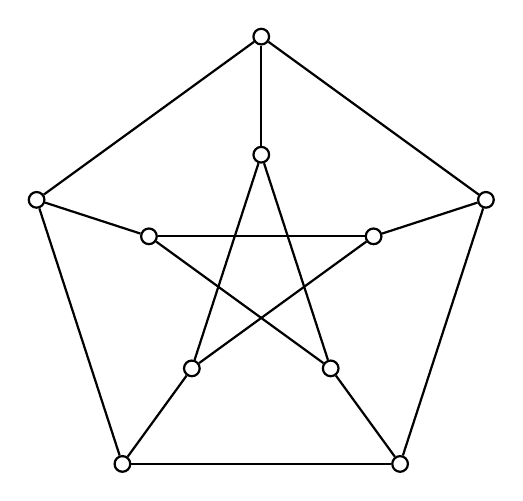
\begin{tikzpicture}
[nodeDecorate/.style={shape=circle,inner sep=2pt,draw,thick},%
  lineDecorate/.style={-,thick},scale=1.5]
%% nodes or vertices
\foreach \nodename/\x/\y in {
  %% outer pentagon
  0/0/2, 1/-1.9021/0.6180, 2/-1.1755/-1.6180, 3/1.1755/-1.6180,
  4/1.9021/0.6180,
  %% inner pentagon
  5/0/1, 6/-0.9510/0.3090, 7/-0.5877/-0.8090, 8/0.5877/-0.8090,
  9/0.9510/0.3090}
{
  \node (\nodename) at (\x,\y) [nodeDecorate] {};
}
%% edges or lines
\path
\foreach \startnode/\endnode in {0/1, 0/4, 0/5, 1/2, 1/6, 2/3, 2/7,
  3/4, 3/8, 4/9, 5/7, 5/8, 6/8, 6/9, 7/9}
{
  (\startnode) edge[lineDecorate] node {} (\endnode)
};
\end{tikzpicture}
\end{figure}

\end{document}
